\tikzset{%
    every neuron/.style={
        circle,
        draw,
        minimum size=5pt,
        inner sep=0pt,
        very thin
    },
    neuron/.style={
        fill
    },
}
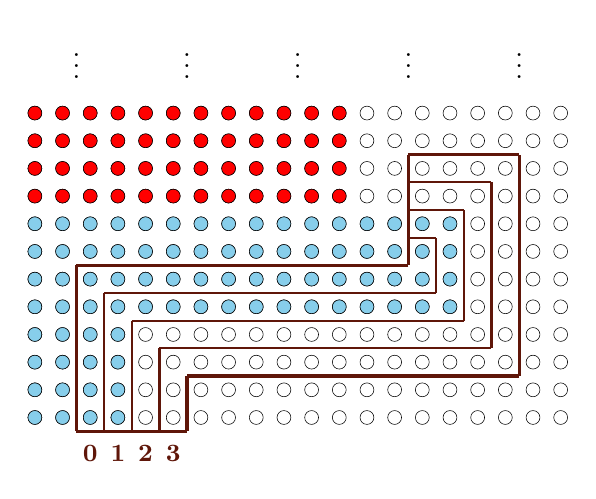
\begin{tikzpicture}[x=0.8cm, y=0.8cm, >=latex, every text node part/.style={align=center}]
    %% BEGIN large grid
    \foreach \x in {0,...,19}
        \foreach \y in {0,...,11} {
        % \foreach \y in {0,...,19} {
            \pgfmathtruncatemacro{\label}{\x*102+\y+3456}
            \node [every neuron/.try] (\label) at (10pt*\x,10pt*\y) {};
        } 
    \foreach \x in {0,...,4}{
        \node [] () at (40pt*\x+15pt, 130pt) {$\vdots$};
    }
    % \foreach \x in {0,...,19}
    %     \foreach \y in {0,...,18} {
    %         \pgfmathtruncatemacro{\label}{\x*102+\y+3456}
    %         \pgfmathtruncatemacro{\labell}{\x*102+\y+1+3456}
    %         \path[very thin] (\label) edge (\labell);
    %     }
    % \foreach \x in {0,...,18}
    %     \foreach \y in {0,...,19} {
    %         \pgfmathtruncatemacro{\label}{\x*102+\y+3456}
    %         \pgfmathtruncatemacro{\labell}{\x*102+\y+102+3456}
    %         \path[very thin] (\label) edge (\labell);
    %     }
    \foreach \x/\y in {0/0, 0/1, 1/1, 2/1, 3/1} 
        \foreach \a in {0,...,3}
            \foreach \b in {0,...,3} {
                \node [every neuron/.try, fill=SkyBlue] () at (40pt*\x + 10pt*\a,40pt*\y + 10pt*\b) {};
            }
    
    % \foreach \x/\y in {0/4, 0/3, 0/2, 1/2, 2/2, 2/3} 
    \foreach \x/\y in {0/2, 1/2, 2/2} 
        \foreach \a in {0,...,3}
            \foreach \b in {0,...,3} {
                \node [every neuron/.try, fill=Red] () at (40pt*\x + 10pt*\a,40pt*\y + 10pt*\b) {};
            }
    %% END large grid

    %% BEGIN large tiles
    \path[Sepia, very thick] (15pt, -5pt) edge (55pt, -5pt);
    \path[Sepia, very thick] (55pt, -5pt) edge (55pt, 15pt);
    \path[Sepia, very thick] (55pt, 15pt) edge (175pt, 15pt);
    \path[Sepia, very thick] (175pt, 15pt) edge (175pt, 95pt);
    \path[Sepia, very thick] (175pt, 95pt) edge (135pt, 95pt);
    \path[Sepia, very thick] (135pt, 95pt) edge (135pt, 55pt);
    \path[Sepia, very thick] (135pt, 55pt) edge (15pt, 55pt);
    \path[Sepia, very thick] (15pt, 55pt) edge (15pt, -5pt);
    %% END lareg tiles

    %% BEGIN sub tiles
    \path[Sepia, thick] (25pt, -5pt) edge (25pt, 45pt);
    \path[Sepia, thick] (25pt, 45pt) edge (145pt, 45pt);
    \path[Sepia, thick] (145pt, 45pt) edge (145pt, 65pt);
    \path[Sepia, thick] (145pt, 65pt) edge (135pt, 65pt);
    
    \path[Sepia, thick] (35pt, -5pt) edge (35pt, 35pt);
    \path[Sepia, thick] (35pt, 35pt) edge (155pt, 35pt);
    \path[Sepia, thick] (155pt, 35pt) edge (155pt, 75pt);
    \path[Sepia, thick] (155pt, 75pt) edge (135pt, 75pt);
    
    \path[Sepia, thick] (45pt, -5pt) edge (45pt, 25pt);
    \path[Sepia, thick] (45pt, 25pt) edge (165pt, 25pt);
    \path[Sepia, thick] (165pt, 25pt) edge (165pt, 85pt);
    \path[Sepia, thick] (165pt, 85pt) edge (135pt, 85pt);

    % \path[Sepia, ->, thick] (15pt, -12.5pt) edge (65pt, -12.5pt);
    % \node [] () at (70pt, -12.5pt) {\small \color{Sepia} $x$};
    % \path[Sepia, ->, thick] (15pt, -12.5pt) edge (-10pt, -37.5pt);
    % \node [] () at (-15pt, -42.5pt) {\small \color{Sepia} $y$};

    \node [] () at (20pt, -13pt) {\small \color{Sepia} \bf 0};
    \node [] () at (30pt, -13pt) {\small \color{Sepia} \bf 1};
    \node [] () at (40pt, -13pt) {\small \color{Sepia} \bf 2};
    \node [] () at (50pt, -13pt) {\small \color{Sepia} \bf 3};

    % \path[Sepia, thick] (20pt, -12.5pt) edge (20pt, -8.5pt); 
    % \path[Sepia, thick] (30pt, -12.5pt) edge (30pt, -8.5pt); 
    % \path[Sepia, thick] (40pt, -12.5pt) edge (40pt, -8.5pt); 
    % \path[Sepia, thick] (50pt, -12.5pt) edge (50pt, -8.5pt); 
    %% END sub tiles
\end{tikzpicture}